\documentclass[12pt]{article}
\usepackage{amssymb}
\usepackage{amsmath}
\usepackage{tikz}
\usetikzlibrary{decorations.markings}

\begin{document}

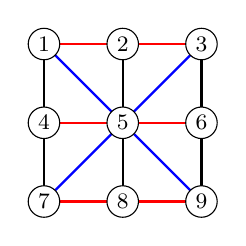
\begin{tikzpicture}[scale=1]
  \draw[thick] (0,0) -- (0,2);
  \draw[thick] (1,0) -- (1,2);
  \draw[thick] (2,0) -- (2,2);
  \draw[red,thick]  (0,0) -- (2,0);
  \draw[red,thick] (0,1) -- (2,1);
  \draw[red,thick] (0,2) -- (2,2);
  \draw[blue,thick] (0,0) -- (2,2);
  \draw[blue,thick] (0,2) -- (2,0);

  \foreach \x in {0,1,2}
  \foreach \y in {0,1,2}
  {
  \draw[fill=white] (\x,\y) circle (0.2cm);
  }
  \fill (0,0) node {\footnotesize 7};
  \fill (0,1) node {\footnotesize 4};
  \fill (0,2) node {\footnotesize 1};
  \fill (1,0) node {\footnotesize 8};
  \fill (1,1) node {\footnotesize 5};
  \fill (1,2) node {\footnotesize 2};
  \fill (2,0) node {\footnotesize 9};
  \fill (2,1) node {\footnotesize 6};
  \fill (2,2) node {\footnotesize 3};
\end{tikzpicture}

\end{document}